\chapter{装饰}

\begin{epigraphe}{《圣经·雅歌》7:10}
    我说,我要上这棕树,抓住枝子。\\愿你的两乳好像葡萄累累下垂,\\你鼻子的气味香如苹果。\\你的口如上好的酒,女子说,\\为我的良人下咽舒畅,流入睡觉人的嘴中。
\end{epigraphe}

那本章的主要思路是介绍,介绍那些为生成文档中个别部分而被个性化修改的\LaTeX 的标准工具,间或可以从中看到些用于``调香''的宏。这些个性化设置可以应用于各个层级:使用包的选项,如设置页眉;偶尔涉足宏定义,如设置章节的展现风格;更深入地处理宏,如处理内容的表格。本章的一部分聚焦于我们可以从包\textsf{fancyvrb}中调用的工具。作为本章的末尾,我们会去抨击一下法文的引号。

\section{索引的外观} % 这节翻译得是什么破玩意

为了修改索引的外观,需要明白,当我们大手一挥噼里啪啦地写下如下指令的时候,我们实际上就生成了一个文件\codereplace{文档}\dm{.ind}:

\dmh{makeindex \codereplace{文档}}

该文件包含了类似下面列出的内容:

\begin{dmd}
\verb|\begin{theindex}| \quad$\leftarrow$\textsf{文前部分}\\
~\\
\verb|\item Cosmic debris, 12,34|\\
~\\
\verb|\indexspace| \quad$\leftarrow$\textsf{分组间的空间}\\
~\\
\verb|\item Debra kadabra, 23| \quad$\leftarrow$\textsf{入口,分割符,页码}\\
~\\
\verb|\end{theindex}| \quad$\leftarrow$\textsf{文后部分}
\end{dmd}

实际上,该代码会从带有预定义值且可被修改的一般性实体中生成。为了证明这个观点,只需要知道,程序\textsf{makeindex}可以生成一个包含\LaTeX 代码外内容的\dm{.ind}文件。为了理解一般性实体的职责,可以用如下方式描述\textsf{makeindex}的工作。

\begin{enumerate}
    \item 根据实体\dm{preamble}的值来写入文前部分。
    \item 对于每个\dm{.idm}文件:
    \begin{enumerate}
        \item 写入实体\dm{item\_0}的内容;
        \item 写入入口(本例中为``Cosmic debris'');
        \item 写入分割符(实体\dm{delin\_0}的值);
        \item 写入页码。
    \end{enumerate}
    \item 在每个分组的结尾(即首字母切换时),写入实体\dm{group\_skip}的内容;
    \item 根据\dm{postamble}的值写入文后部分。
\end{enumerate}

上述实体的默认值如下:

\begin{center}
    \begin{dmd}
        \begin{tabular}{|l|l|}
            \hline
            preamble & \verb+"\\begin{theindex}\n"+\\
            item\_0 &\verb+"\n \\item"+\\
            delim\_0 & ", "\\
            group\_skip & \verb+"\n\n \\indexspace\n"+\\
            postamble & \verb+"\n\n\\end{theindex}\n"+\\
            \hline
        \end{tabular}
    \end{dmd}
\end{center}

这些值可以使用通常带有后缀名\dm{.ist}的风格文件作为媒介来修改。可以通过以下方式在调用\textsf{makeindex}时使用:

\dmh{makeindex -s \codereplace{风格}.ist \codereplace{文件}}

如此一来,为了生成文档的标题,我们可以一开始就重新定义一二级间的分隔符:

\begin{dmd}
\begin{verbatim}
delim_0 " \\dotfill \ "
delim_1 " \\dotfill \ "\end{verbatim}
\end{dmd}

我们将默认用于分隔索引入口和页码的逗号替换成了省略号。接下来,通过严谨地阅读\textsf{makeindex}的文档\jz{
    可参见参考文献的实用引用后的提醒。
},可以注意到要求\textsf{makeindex}为入口组和代表分组的字母间生成空间的礼貌方式如下:

\begin{dmd}
headings\_flag 1
\end{dmd}

这里,代表分组的字母会表示为大写,并且借助实体\dm{heading\_prefix}和\dm{heading\_suffix}的内容框起。无所谓——为了生成我们美丽的带阴影的字盒,我们可以在风格文件中这样写:

\begin{dmd}
\begin{verbatim}
heading_prefix "{\\large\\sffamily\\bfseries\\shadowbox{"
heading_suffix "}\\hfill}\\nopagebreak\n"\end{verbatim}
\end{dmd}

这段你已经可以看懂的示例内容,就会生成我们需要的字盒。例如对于字母C:

\begin{codelist}[10.1]{
    {\large\sffamily\bfseries%
    \shadowbox{C}\hfil}\nopagebreak
}
\begin{verbatim}
{\large\sffamily\bfseries%
    \shadowbox{C}\hfil}\nopagebreak\end{verbatim}
\end{codelist}

这段指令会被\dm{group\_skip}的内容覆盖掉。而我们稍早前说过,\dm{group\_skip}的默认值是\verb|\indexspace|。在研究了几个月之后\jz{
    开玩笑的。我是想说,只花了几秒……好吧,几分钟。
},我们成功地在\dm{book.cls}中发现了该指令的定义,并且将分组间空间略微扩大了些:

\begin{dmd}
\renewcommand\indexspace{%
    \par \vskip 20pt plus5pt minus3pt\relax}
\end{dmd}

\begin{ii}
本小节中,我们只是非常简单地看了看makeindex提供的功能。除了在《\LaTeX 伴侣》中能找到的信息,Debian环境下关于此工具的说明书中提供了我们可以定义的一半入口的详尽列表。由P.陈(P. Chen;音译)和M.A.哈林森(M. A. Harrinson)编写的文件\dm{ind.dvi}同样是初学索引自定义的良好开端。
\end{ii}

\section{标题的外观}

在本节,我们会介绍我们修改\LaTeX 标准(篇、章、节等)标题外观的方式。

\subsection{目录中的编号}

作为开始操作目录的前提条件,需要掌握两个计数器:

\begin{enumerate}
    \item \dm{secnumdepth}(英:\emph{section numbering depth}),可以明确文档中标题编号的层级;
    \item \dm{tocdepth}(英:\emph{table of contents depth}),可以定义目录标题的最大层级(或称最大深度)。
\end{enumerate}

为了使用这两个计数器,还需要了解\LaTeX 为各标题连接层级的方法。以下是各标题的层级:

\begin{center}
    \begin{tabular}{|c|r||c|r|}
        \hline
        标题 & 层级 & 标题 & 层级\\
        \hline
        \dm{part} & -1 & & \\
        \dm{chapter}    & 0 & \dm{subsubsection} & 3\\
        \dm{section}    & 1 & \dm{paragraph}     & 4\\
        \dm{subsection} & 2 & \dm{subparagraph}  & 5\\
        \hline
    \end{tabular}
\end{center}

如此一来,将\verb|secnumdepth|赋值为1、将\verb|tocdepth|赋值为2,则可以让标题编号至各\verb|\section|,同时将层级少于\verb|\subsection|的标题插入目录。

\subsection{节和更少的层级}

在\TeX 系统的文件\dm{book.cls}中,我们可以找到如下代码\jz{
    稍微简化了一些……
}:

\begin{dmd}
\begin{verbatim}
\newcommand{\section}{%
    \@startsection%
    {section} % 标题名称
    {1} % 标题层级
    {0pt} % 缩进
    {-3.5ex plus -1ex minus -.2ex}% 段前纵向空间
    {2.3ex plus.2ex}% 段后纵向空间{\normalfont\Large\bfseries}} % 标题外观\end{verbatim}
\end{dmd}

该段代码定义了节标题的生成方式。可以观察到,指令\verb|\section|调用了指令\verb|\@startsection|,而后者需要6各参数:

\begin{itemize}
    \item 标题名称,如\dm{section}、\dm{subsection}等;
    \item 标题层级,1对应\dm{section},2对应\dm{subsection},3对应\dm{subsubsection},等等;
    \item 缩进;
    \item 标题前的纵向空白;
    \item 标题后的纵向空白;
    \item 用于确定标题本身格式的一系列\emph{声明}。
\end{itemize}

因此,我们可以注意到\LaTeX 默认为类型\dm{book}设定的版式如下。

\begin{itemize}
    \item 无缩进(\dm{0pt})。
    \item 标题前的纵向空间为\dm{3.5ex},带有正向\dm{-1ex}和负向\dm{-.2ex}的允差。
    \item 标题后的纵向空间为\dm{2.3ex},带有正向\dm{.2ex}的允差。可以注意到,如果空间为负,则段落开头会紧接标题,而不会重起一段。
    \item 标题加粗加大,使用``常规''(normal)字体。
\end{itemize}

为了定义本文档使用的标题样式,我们引入三个长度,分别用于\dm{section}、\dm{subsection}、\dm{subsubsection}的缩进:

\begin{dmd}
\begin{verbatim}
\newlength{\sectiontitleindent}
\newlength{\subsectiontitleindent}
\newlength{\subsubsectiontitleindent}\end{verbatim}
\end{dmd}

长度值如下:

\begin{dmd}
\begin{verbatim}
\setlength{\sectiontitleindent}{-1cm}
\setlength{\subsectiontitleindent}{-.5cm}
\setlength{\subsubsectiontitleindent}{-.25cm}\end{verbatim}
\end{dmd}

此外,我们为标题还定义了特殊的字体,具体如下:

\begin{dmd}
\begin{verbatim}
\newcommand{\sectionfont}{% 
    \fontencoding{\encodingdefault}% 
    \fontfamily{pag}% \fontseries{bc}%
    \fontshape{n}% \selectfont}\end{verbatim}
\end{dmd}

该指令可以选用PostScript字体AvantGarde的加粗紧缩版本(参阅9.4节)%TODO 解释中文的使用
。最终,我们使用了以下指令来定义节标题外观:

\begin{dmd}
\begin{verbatim}
\renewcommand{\section}{% 
    \@startsection%
    {section}%
    {1}%
    {\sectiontitleindent}%
    {-3.5ex plus -1ex minus -.2ex}% 
    {2.3ex plus.2ex}% {\sectionfont\Large}}\end{verbatim}
\end{dmd}

对于更少层级的标题,我们也编写了等价的指令。

\subsection{章}

通过深入研究文件\dm{book.cls},我们可以找到有关\LaTeX 生成章首内容的信息。

\subsubsection{原则}

在文件\dm{book.cls}中,我们可以找到以下指令:

\begin{dmd}
\begin{verbatim}
\newcommand{\chapter}{% 
    ...
    \thispagestyle{plain}%
    ...
    \secdef\@chapter\@schapter} % 我们感兴趣的行\end{verbatim}
\end{dmd}

指令\verb|\chapter|本身会调用两个不同的指令:

\begin{enumerate}
    \item \verb|\@chapter|,用于被编号的章标题;
    \item \verb|\@schapter|,用于不被编号的章标题(\dm{s}代表\emph{star},即``星号'',对应指令\verb|\chapter*|)。
\end{enumerate}

在英勇地(同样在文件\dm{book.cls}中)查找这两条指令的定义之后,我们找到了下面这类东西:

\begin{dmd}
\begin{verbatim}
\def\@chapter[#1]#2{% ...
    \refstepcounter{chapter}%
    % 终端上的消息:
    \typeout{\@chapapp\space\thechapter.} 
    \addcontentsline{toc}{chapter}% 在目录中添加标题
    ...
    \if@twocolumn
    ...
    \else% 针对不分栏的文档
    \@makechapterhead{#2}% 我们感兴趣的代码行
    \fi}\end{verbatim}
\end{dmd}

这段代码把我们领上道了……实际上,\verb+\@makechapterhead+(可以按字面翻译为``制作章首装饰'')正是我们更改图案所需要重定义的指令。经过进一步的搜索,我们可以发现指令\verb|\@makeschapterhead|能够生成未编号的章首装饰。这两条指令接受章名作为其参数。

\subsubsection{必要的小工具}

我们定义了环境\dm{cadrechap},用于简单地讲右边距加宽2厘米:

\begin{dmd}
\begin{verbatim}
\newenvironment{cadrechap}% 
    {\begin{list}{}{%
        \setlength{\leftmargin}{0pt}% 
        \setlength{\rightmargin}{-2cm}% 宽敞些
        \setlength{\itemindent}{0pt}% 
        \setlength{\labelsep}{0pt}%
    }\item}% 
{\end{list}}\end{verbatim}
\end{dmd}

同时,可以使用布尔值\dm{@mainmatter}来获取我们目前是否处于文档的``中心''——这是针对指令\verb|\mainmatter|被调用的情况。

\subsubsection{严格的章首装饰}

本文档中,生成章首装饰的指令可以看作两个微型页面的组合。%TODO minipage

\begin{enumerate}
    \item 在左侧的是微型页面字盒。我们指定了它的高度,以便放置微型摘要(参见\S 10.7)。
    \item 在右侧的是包含``章''一词和章号的字盒。
\end{enumerate}

\newcommand{\boite}[1]{%
  {\setlength{\fboxrule}{.2pt}%
    \setlength{\fboxsep}{-\fboxrule}%
    \fbox{#1}}}
\DeclareFixedFont{\fnumfont}{T1}{phv}{b}{n}{32pt}
\DeclareFixedFont{\fnomfont}{T1}{phv}{b}{n}{12pt}
\DeclareFixedFont{\ftitrefont}{T1}{phv}{b}{n}{16pt}

\newcommand{\fairechapitre}[1]{%
  \noindent\begin{minipage}{\linewidth}%
      \boite{\begin{minipage}[t][3cm][c]{.75\textwidth}%
          \centering%
          为\\微型摘要\\准备的\\微型页面
        \end{minipage}}%
      \boite{\begin{minipage}[t]{.25\textwidth}
          \begin{flushright}
            {\fnomfont\chaptername}\\[.5cm]
            {\fnumfont\thechapter}
          \end{flushright}
        \end{minipage}}
    \end{minipage}\par
  \begin{flushright}\ftitrefont#1\end{flushright}}

\fairechapitre{Zhang biaoti}%TODO  font

实现此类字盒组合的框架如下:

\begin{dmd}
\begin{verbatim}
\begin{cadrechap}
    \begin{minipage}[t][6cm][t]{0.75\linewidth}
        % 这里插入微型摘要 
    \end{minipage} 
    \begin{minipage}[t]{0.25\linewidth}
        % 这里插入章号
    \end{minipage}
    \begin{flushright}
        % 这里插入章标题
    \end{flushright}
\end{cadrechap}\end{verbatim}
\end{dmd}

此处无疑需要注意到,左侧的字盒(即接收微型目录的字盒)带有可指定的高度,用于以一致的方法来生成章首装饰而无须关注章中的节数(即无须关注微型目录的高度)。接下来,为不同元素定义不同的字体,就可以完成章首装饰的定义。在本文档中,我们的定义如下:

\begin{dmd}
\begin{verbatim}
% 章号
\DeclareFixedFont{\chapnumfont}{T1}{phv}{b}{n}{80pt}
% ``章''一词
\DeclareFixedFont{\chapchapfont}{T1}{phv}{b}{n}{16pt}
% 章标题
\DeclareFixedFont{\chaptitfont}{T1}{phv}{b}{n}{24.88pt}\end{verbatim}
\end{dmd}

\DeclareFixedFont{\chapnumfont}{T1}{phv}{b}{n}{80pt}
\DeclareFixedFont{\chaptitfont}{T1}{phv}{b}{n}{24.88pt}

因此,有如下指令:

\begin{codelist}[10.2]{
    {\chapnumfont 8}
    {\chaptitfont Oula !}
}
\begin{verbatim}
{\chapnumfont 8}
{\chaptitfont Oula !}\end{verbatim}
\end{codelist}

\subsection{部分}

在文件\dm{book.cls}中,我们可以找到指令\verb|\part|的定义:

\begin{dmd}
\begin{verbatim}
\newcommand\part{% 
    \cleardoublepage
    \thispagestyle{plain}
    [...]
    \null\vfil
    \secdef\@part\@spart}\end{verbatim}
\end{dmd}

该定义告诉我们,正如各章一样,指令\verb|\part|会调用两条独立的指令,用于生成编号和不编号的部分(分别借助指令\verb|\@part|和\verb|\@spart|)。在之前的实践中,我们指定了页面的风格,使得各部分的开头为空(即没有页码和部分开头的装饰等),指令如下:

\begin{dmd}
\begin{verbatim}
\newcommand\part{%
    \cleardoublepage
    \thispagestyle{empty}% 代替默认的plain
    [...]
    \null\vfil% 空字盒和竖直方向的弹性空间
    \secdef\@part\@spart}\end{verbatim}
\end{dmd}

接下来,我们可以查看指令\verb|\@part|的定义。该指令用于生成展示文档部分的页:

\begin{dmd}
\begin{verbatim}
\def\@part[#1]#2{%
    [...]
    {\centering % 居中
     [...]
     \huge\bfseries \partname\nobreakspace\thepart
        \par
        \vskip 20\pt
     [...]
     \Huge \bfseries #2\par}% 
\@endpart}\end{verbatim}
\end{dmd}

通过查看这段代码,我们了解到,展现部分的页面由一行加粗加大的``部分''字样和部分的序号构成\jz{
    实际上,在联动了包\textsf{babel}和选项\dm{french}后,这两个指令会被重定义,以生成形如``Première partie''(第一部分)的内容。
}:

\begin{dmd}
\verb|\huge\bfseries \partname\nobreakspace\thepart|
\end{dmd}

在距离20点的下方,是部分的标题(存储在参数\verb|#2|中)。对于此文档,我们以如下方式重定义了指令\verb|\@part|:

\begin{dmd}
\begin{verbatim}
\def\@part[#1]#2{% 
    [...]
    {\centering
     \interlinepenalty \@M
     \normalfont
     [...]
     \partnumfont \thepart % 只显示部分的序号
     \par
     \vskip 50\p@% 将20点改为50点
     \partfont #2\par}% 使用自定义字体的标题
    \@endpart}\end{verbatim}
\end{dmd}

为了与章首装饰保持一致,我们定义指定字体的指令如下:

\begin{dmd}
\begin{verbatim}
\newcommand{\partfont}{% 
    \fontencoding{\encodingdefault}\fontfamily{phv}% 
    \fontseries{bc}\fontshape{n}% \fontsize{32}{34}%
    \selectfont}
\DeclareFixedFont{\partnumfont}{T1}{phv}{bc}{n}{80}%\end{verbatim}
\end{dmd}

\begin{exclamation}
我们也应注意到,指令\verb+\@part+依靠调用另一条指令作为结尾:\verb|\@endpart|。通过查看文件\dm{book.cls}可以看到,这样的结尾可以阻止来自指令\verb|\part|的纵向弹性空间,并跳过一个空白页……
\end{exclamation}

\section{几何}

本文档中,各页面中的不同尺寸借助包\textsf{geometry}使用如下指令定义:

\begin{dmd}
\begin{verbatim}
\geometry{%
    a4paper, 
    body={150mm,250mm}, 
    left=25mm,top=25mm, 
    headheight=7mm,headsep=4mm, marginparsep=4mm, 
    marginparwidth=27mm}\end{verbatim}
\end{dmd}

这会分别定义如下元素(如图\ref{fig:10.1}所示):

\begin{itemize}
    \item 版心宽150 mm,高250 mm;
    \item 版心在页面上的位置为左边距25 mm、上边距25 mm;
    \item 页眉高7 mm,页眉与正文的间距为4 mm;
    \item 页面尺寸为标准A4;
    \item 用于页边注释的页边距为2.7 cm。
\end{itemize}

\begin{figure}[ht]
    \centering
    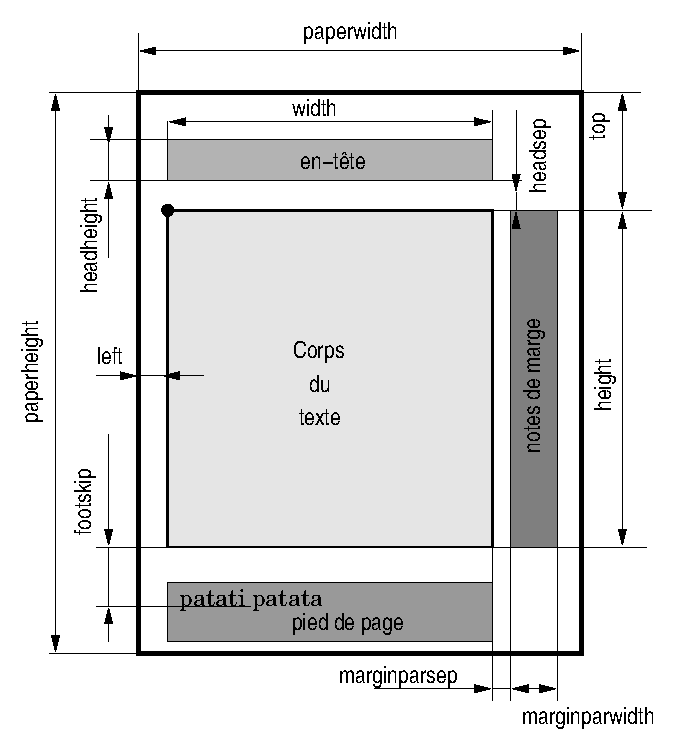
\includegraphics{img/geometry}
    \caption{定义文档几何样式的部分尺寸}
    \label{fig:10.1}
\end{figure}

以通常的方式来讲,正如图\ref{fig:10.1}展现的,包\textsf{geometry}可以定义一定数量的尺寸。我们可以以选项的方式将这些尺寸传递给\verb|\usepackage|,也可以借助指令\verb|\geometry|。

\begin{description}
    \item[页面尺寸]%TODO 此处如何换行,下同
    
\begin{itemize}
    \item 若使用预定义中的格式,可以使用\dm{a4paper}、\dm{a5paper}等。
    \item 若要自由地指定纸张尺寸,例如针对会使用碎纸机销毁的文档的尺寸,可以使用\dm{paperwidth=}\codereplace{尺寸}和\dm{paperheight=}\codereplace{尺寸}。
\end{itemize}

\item[文本]

\begin{itemize}
    \item 可以使用\dm{body=\{\codereplace{宽度},\codereplace{高度}\}};
    \item 也可以使用\dm{width=}\codereplace{宽度}和\dm{height=}\codereplace{高度};
    \item 文本在页面内的位置由参考点确定,可以使用\dm{top=}\codereplace{纵向位置}和\dm{left=}\codereplace{水平位置}确定参考点位置。
\end{itemize}

\item[页面顶端和底部]

\begin{itemize}
    \item 页面中为页面预留的高度可以借助神奇的表达式\dm{headheight=}\codereplace{高度}定义,页眉相对于版心的位置可以借助指令\dm{headsep=}\codereplace{空间}指定;
    \item 页脚的位置可以通过长度\dm{footskipp=}\codereplace{空间}指定,该长度可以定义版心底部和页脚第一行间的空间。
\end{itemize}

\item[页边注释] 秉承着同样的精神,页面中为边注预留的空间的宽度和位置可以借助两个长度定义:\dm{marginparwidth=}\codereplace{宽度}和\dm{marginparsep=}\codereplace{空间}
\end{description}

\begin{exclamation}
包geometry中,涉及页眉、页脚、边注的尺寸默认算作版心\emph{外}的部分。有一些指令可以将这些尺寸中的一个或多个包含到版心内部来完成计算。例如,我们可以说``我希望版心宽度为10厘米,包含边注''。关于更多相关细节,请参阅包文档。
\end{exclamation}

\section{页眉和页脚}

版心上下的空间分别成为页眉和页脚,可以借助包\textsf{fancyhdr}来定制。定制的基本原则很简单\jz{
    在读完接下来的内容后,你无疑会开始质疑这里说的``简单''一词……
},只需要使用以下指令来指明我们想要使用借助包\textsf{fancyhdr}定义的页眉和页脚。该包默认会在页面下方和页脚上方生成一条水平线段,线段粗细分别由\verb|\footrulewidth|和\verb|\headrulewidth|定义。接下来,我们使用以下指令:

\begin{itemize}
    \item \verb|\fancyhead|,来定义页眉;
    \item \verb|\fancyfoot|,来定义页脚。
\end{itemize}

这两条指令都可以接收由一个或两个以下字符组成的序列构成的参数:

\begin{itemize}
    \item \dm{E}或\dm{O},用于指明页码的奇偶性(偶数即\emph{even},奇数即\emph{odd});
    \item \dm{R}、\dm{L}或\dm{C},用于指明我们想在哪个位置生成信息,分别指代右侧、左侧或居中。
\end{itemize}

示例如下:

\begin{dmd}
\begin{verbatim}
\fancyhf{} % 清除页面并开始
% 【页眉】
% 作者姓名首字母偶数页靠右,奇数页靠左:
\fancyhead[RE,LO]{VL}
% 页码居中:
\fancyhead[C]{\thepage}
% 节号奇数页靠右,
% 偶数页靠左:
\fancyhead[LE,RO]{\thesection}
% 【页脚】
% 图片奇数页靠右,偶数页靠左:
\fancyfoot[RO,LE]{
\includegraphics[height=4ex]{punch}}
% 标题奇数页靠右,偶数页靠左:
\fancyfoot[LO,RE]{%
    关于\LaTeX{}的那些你想知道的问题}
% 线条粗细
\renewcommand{\footrulewidth}{3pt}\end{verbatim}
\end{dmd}

\fancyhf{} 
\fancyhead[RE,LO]{VL}
\fancyhead[C]{\thepage}
\fancyhead[LE,RO]{\thesection}
\fancyfoot[RO,LE]{
\includegraphics[height=4ex]{punch}}
\fancyfoot[LO,RE]{关于\LaTeX{}的那些你想知道的问题}
\renewcommand{\footrulewidth}{3pt}

\subsection{章首页的情况}

在类型\dm{book}中,\LaTeX 会自动为每章的第一页调用风格\dm{plain}。为了使包\textsf{fancyhdr}为这些页面定义新风格,可以使用如下指令:

\begin{dmd}
\begin{verbatim}
% 章首页的情况 
\fancypagestyle{plain}{%
    \fancyhf{}% 全部清空 
    \fancyfoot[C]{\thepage}% 页面底部的页码
    % 清空所有线条
    \renewcommand{\headrulewidth}{0pt}% 
    \renewcommand{\footrulewidth}{0pt}}\end{verbatim}
\end{dmd}

可以注意到,本书各章的章首正是采用了这种风格……

\subsection{章首前的空白页}

在类型\dm{book}的双面模式下(正是本文档对应的情况),\LaTeX 会默认在奇数页——这在排版术语中称作``单面''(belle page)——开始新的一章。为了实现这一点,\LaTeX 在不同的内部指令中调用了指令\verb+\cleardoublepage+。这样可以在必要时在章的首页前插入一个空白页。默认情况下,该空白页会带有目前使用的页眉和页脚。在本文档中,我们针对这些页面修改了文件\dm{latex.ltx}中的指令\verb|\cleardoublepage|,指定了一种``空白''的风格:%TODO 还没搞

\begin{dmd}
\begin{verbatim}
\renewcommand{\cleardoublepage}{% 重定义该指令
    \clearpage\ifodd\c@page\else
    \hbox{}
    \vspace*{\fill}
    \thispagestyle{empty}% 添加此行 
    \newpage
    \fi}\end{verbatim}
\end{dmd}

你可以翻阅本书,看看章首前的页面是否是空白的……

\subsection{标记的机制}

你无疑已经注意到了,本书的页眉带有一些与文本相关的内容。实际上,针对偶数页(出现在左侧的页面),我们插入了章标题;针对奇数页(出现在右侧的页面),我们插入了该页出现的最后一节的节标题。\LaTeX 部署了一种\emph{标记}机制,使得我们可以实现这一点。这里将尝试解释这种机制。

\begin{exclamation}
这里不妨解释一下:\LaTeX 和\TeX 生成一个页面是,它们会根据从所涉页面收集来的信息来制备页眉和页脚。因此,生成页眉和页脚是编译页面的后置步骤。
\end{exclamation}

\subsubsection{指令\dm{\backslash markboth}和\dm{\backslash markright}}

设有以下指令:

\begin{dmd}
\backslash markboth\{\codereplace{文本$_{\mbox{左}}$}\}\{\codereplace{文本$_{\mbox{右}}$}\}
\end{dmd}

或:

\begin{dmd}
\backslash markright\{\codereplace{文本}\}
\end{dmd}

想象参数\codereplace{文本$_{x}$}存储在栈和队列中。根据这种想法,有:

\begin{itemize}
    \item \verb|\markboth|将\codereplace{文本$_{\mbox{左}}$}入栈,将\codereplace{文本$_{\mbox{右}}$}存入队列;
    \item \verb|\markright|将\codereplace{文本}存入队列。
\end{itemize}

在一个页面中,这两个``标记''指令可以调用多次,也可以一次都不调用。在\TeX 结束版心的排版,在生成页眉和页脚时,会探索栈和队列的参数。这借助了以下指令:

\begin{itemize}
    \item \verb|\leftmark|返回栈顶,即\emph{上一次调用}\verb|\markboth|时的\codereplace{文本$_{\mbox{左}}$};
    \item \verb|\rightmark|返回队列头,即\emph{第一次调用}\verb|\markboth|时的\codereplace{文本$_{\mbox{右}}$},或\emph{第一次调用}\verb|\markbot|时的\codereplace{文本}。
\end{itemize}

\begin{exclamation}
我们这里介绍的``队列''有一个小巧思:只要页面中没有``标记''指令添加数据,那么队列就会保持此前的页面中\emph{最后插入的信息}。指令\verb|\markboth|和\verb|\markright|一出现,``队列''就被清空。
\end{exclamation}

另一个理解这种标记机制的方法可以描述如下:

\begin{itemize}
    \item \verb|\leftmark|包含入栈的最后一条信息(借助\verb|\markboth|的第一个参数);
    \item 如果我们在页面上放置了一词\verb|\rightmark|,则它包含``队列''的第一条信息,否则它包含队列中的最后一条信息(借助\verb|\markboth|的第二个参数或\verb|\markright|的参数)。
\end{itemize}

\begin{ii}
    供你参考的是,作者使用了这些指令来生成了带有几十个名称和照片的相册。这里的思路是去探索通过页眉显示页面上第一个和最后一个名称的机制——这种页眉跟字典很像。为了实现这个目的,只需要为每个人(包含名称和照片)调用以下指令:
    
    \begin{dmd}
    \backslash markboth\{\codereplace{老铁的名称}\}\{\codereplace{老铁的名称}\}
    \end{dmd}
    
    接下来,在左侧页面页眉中插入指令\verb|\rightmark|,在右侧插入\verb|\leftmark|……
\end{ii}

\subsubsection{与段落指令的互动}

在各章、节、小节等结构的开头,\LaTeX 的一条内部指令会调用前文介绍过的标记指令,以将疑似可以丰富页眉和页脚内容的信息存储起来。这些指令的名称如下:

\begin{itemize}
    \item \verb|\chaptermark|,适用于章;
    \item \verb|\sectionmark|,适用于节;
    \item ……
\end{itemize}

这些指令会等待包含章或段落标题的参数。对于本书,前面列出的两条指令采用如下方式定义:

\begin{dmd}
\begin{verbatim}
% #1包含节标题
\renewcommand{\sectionmark}[1]{%
    \markright{\sectionfont\thesection\ #1}}
% #2 包含章标题
\renewcommand{\chaptermark}[1]{%
    \markboth{\sectionfont#1}{}}\end{verbatim}
\end{dmd}

接下来有:

\begin{dmd}
\begin{verbatim}
\fancyhead[LE,RO]{\thepage}
\fancyhead[LO]{\rightmark}
\fancyhead[RE]{\leftmark}\end{verbatim}
\end{dmd}

这样一来:

\begin{itemize}
    \item 在偶数页的右侧,我们可以找到上一个章标题(\verb|\leftmark|);
    \item 在奇数页的左侧,我们可以找到当前页的第一个\verb|\section|,包含序号和标题,或是上一个\verb|\section|的序号和标题(\verb|\rightmark|)……
\end{itemize}

%TODO 对于前置页面的单章双节?

\fancyhf{}
% \fancyhead[LE]{\bfseries\thepage}
% \fancyhead[RO]{\bfseries\thepage}
\fancyhead[LE]{\ongletpaire\bfseries\thepage}
\fancyhead[RO]{\bfseries\thepage\ongletimpaire}
\fancyhead[LO]{\texttt{\backslash rightmark}的值为``\rightmark{}'',\texttt{\backslash leftmark}的值为``\leftmark''}
\fancyhead[RE]{\texttt{\backslash rightmark}的值为``\rightmark{}'',\texttt{\backslash leftmark}的值为``\leftmark''}
\renewcommand{\footrulewidth}{0pt}

如果你不相信,可以亲自看看本章的页眉。

\subsection{文档的组织}

需要知道,对于形如本书的文档,\LaTeX 可以识别出三大部分,在英文中分别称作\emph{front matter}、\emph{main matter}和\emph{back matter},分别代表文章的开头(通常带有前言和摘要)、作为主体的部分、用于收尾的部分(通常带有目录、附录、参考文献、术语字典等)。因此,我们应该明确,\LaTeX 文档的书写形式如下:

\begin{dmd}
\backslash documentclass\{\codereplace{文档类型}\}
\begin{verbatim}
\begin{document}
\frontmatter % 前言
[...]
\mainmatter % 主体部分
[...]
\backmatter % 用于收尾
[...]
\end{document}\end{verbatim}
\end{dmd}

接下来,我们将会着手逐一修改这三个指令。目前你需要知道的是,类型\dm{book}种定义了一个布尔值:

\begin{dmd}
\verb|\newif\if@mainmatter|
\end{dmd}

\LaTeX 默认使用该值来获取当前我们是否处于``main matter''中。此外,我们的文档中还有另一个布尔值:

\begin{dmd}
\verb+\newif\if@frontmatter+
\end{dmd}

该值可以使我们为文档中介绍性的部分进行特殊处理。界定三大部分的三个指令定义如下:

\begin{dmd}
\begin{verbatim}
\renewcommand\frontmatter{%
    \cleardoublepage
    \@frontmattertrue
    \@mainmatterfalse
    \pagenumbering{roman}% 以罗马数字编号
}
\renewcommand\mainmatter{%
    \cleardoublepage
    \@mainmattertrue
    \@frontmatterfalse
    \pagenumbering{arabic}% 以阿拉伯数字编号
}
\renewcommand\backmatter{%
    \cleardoublepage
    \@frontmatterfalse
    \@mainmatterfalse
}\end{verbatim}
\end{dmd}

在\LaTeX 源代码中一番翻找后,我们就可以明白,指令\verb|\pagenumbering|能够修改编号方式,并且将页码计数器重置为1。

%
% TODO on remet tous commme c'�tait avant
%
\fancyhf{}
% \fancyhead[LE]{\bfseries\thepage}
% \fancyhead[RO]{\bfseries\thepage}
\fancyhead[LE]{\ongletpaire\bfseries\thepage}
\fancyhead[RO]{\bfseries\thepage\ongletimpaire}
\fancyhead[LO]{\bfseries\rightmark}
\fancyhead[RE]{\bfseries\leftmark}
\renewcommand{\footrulewidth}{0pt}

\subsection{以``小型大写''罗马数字为前言编号}

鄙人坚持认为,前言部分的页码应当以小型大写罗马数字标示。很不幸,我们不能写成这样:

\begin{dmd}
\verb|\renewcommand{\thepage}{\textsc{\roman{page}}}|
\end{dmd}

这是因为,这样的写法会导致索引的不兼容。这里的思路是按如下步骤处理:

\begin{enumerate}
    \item 使用小写罗马数字编号;
    \item 在页脚显示\verb|\textsc{\thepage}|;
    \item 修改指令\verb|\index|来使页码显示为小型大写。
\end{enumerate}

这样一来,我们需要在\verb|\frontmatter|的定义中添加如下内容:

\begin{dmd}
\begin{verbatim}
\let\indexORI\index% 保存初始的定义
\renewcommand{\index}[1]{\indexORI{##1|textsc}} 
\fancyfoot{}
\fancyhead[LE,RO]{\textsc{\thepage}}\end{verbatim}
\end{dmd}

在\verb|\mainmatter|的定义中添加如下内容:

\begin{dmd}
\begin{verbatim}
\let\index\indexORI% 以回到初始的定义\end{verbatim}
\end{dmd}

为了完美地达到我们的严格标准,我们也会修改章首页的风格:

\begin{dmd}
\begin{verbatim}
\fancypagestyle{plain}{% 
    \fancyhf{}
    \if@frontmatter% 前言
        \fancyfoot[C]{\textsc{\thepage}}
    \else
        \fancyfoot[C]{\thepage}
    \fi
    \renewcommand{\headrulewidth}{0pt}
    \renewcommand{\footrulewidth}{0pt}}
\makeatother\end{verbatim}
\end{dmd}

\subsection{索引、参考文献和目录}

在类型\dm{book}中,定义了两种环境:

\begin{itemize}
    \item \dm{thebibliography},用于生成参考文献;
    \item \dm{theindex},用于生成索引。
\end{itemize}

此外,还定义了一个指令:

\begin{itemize}
    \item \verb|\tableofcontents|,用于生成目录。
\end{itemize}

这些环境或指令被设计为可以生成带有页码和大写标题的页眉,即\verb|\bibname|、\verb|\indexname|和\verb|\contentsname|。例如,以下是\verb|\tableofcontents|的节选:

\begin{dmd}
\begin{verbatim}
\newcommand\tableofcontents{% 
    [...]
    \chapter*{\contentsname 
        \@mkboth{%
            \MakeUppercase\contentsname}% 
           {\MakeUppercase\contentsname}}%
    \@starttoc{toc}% 
    [...]
}\end{verbatim}
\end{dmd}

我希望本文档的页眉不采用大写形式。有采用两种解决方式。

\begin{itemize}
    \item 使用包\textsf{fancyhdr}的指令\verb|\nouppercase|,并在\verb|\backmatter|的定义中编写如下内容:
    \begin{dmd}
    \begin{verbatim}
% 大写页眉: 
\fancyhead[LO]{\nouppercase\rightmark} 
\fancyhead[RE]{\nouppercase\leftmark}%
    \end{verbatim}
    \end{dmd}
    
    \item  重新复制并修改源于\dm{book.cls}的宏\verb|\tableofcontents|,将其中多次出现的指令\verb|\MakeUppercase|全部删除。对于索引和参考文献进行相同的操作。
\end{itemize}

本文档采用了第二种方式。我们同样在目录中插入索引和参考文献时,也同样可以感受到这种方式带来的优势——默认情况下,\LaTeX 和类型\dm{book}对此不兼容。因此,我们有了如下形式的环境\dm{theindex}:

\begin{dmd}
\begin{verbatim}
\renewenvironment{theindex} {%
    [...]
    % 插入至目录
    \addcontentsline{toc}{chapter}{\indexname}
    % 删除\MakeUppercase
    \@mkboth{\indexname}{\indexname}
    \thispagestyle{plain}
    [...]
{\if@restonecol\onecolumn\else\clearpage\fi}\end{verbatim}
\end{dmd}

\section{``照抄''环境}

包\textsf{fancyvrb}和\textsf{listings}都包含可以生成带特殊符号文本的特性。其中,前者更加灵活,可以生成\dm{verbatim}种类的环境,特别是可以定制必要的边框和边距。最重要的是,它允许你从环境的正中央``逃回\LaTeX '',或者按英语国家的人所说的:\emph{to escape to \LaTeX }。换句话说,尽管是在符号\verb|\|、\dm{\{}、\dm{\}}都不起作用的环境中,我们仍然可以调用\LaTeX 的指令。

后者(\textsf{listings})致力于生成代码片段。它提供的大量功能中,同样包含可以逃回\LaTeX 的方法。这里我们推荐你借助本章使用的``真实复刻''示例探索一下这两个环境。

\subsection{跑个题,说说符号……}

在这里我想先说说\TeX 如何``消化吸收''我们喂给它的字符——我相信这题没有白偏\jz{
    在做事低调这件事上,法国人似乎是专家,但我们不要偏太远了……
}。需要明白,符号可以被划分为16中类别,每个符号只能同时属于其中的一种。每种类别都可以由\TeX 特殊处理。例如,遇到符号\dm{\backslash}时,\TeX 会读取其后面的字符组,来识别指令(或\emph{控制序列})的名称;遇到符号\dm{\{}时,\TeX 会开启新的组;读取到符号\dm{\%}时,\TeX 会一路忽略接下来符号,直到当前行结束,也就是遇到标记``行末''的符号,等等。\TeX 可以识别的类别举例如下:

\begin{description}
    \item[类0]控制符号(\LaTeX 中的\dm{\backslash});
    \item[类1]组起始符号(\LaTeX 中的\dm{\{});
    \item[类2]组结束符号(\LaTeX 中的\dm{\}});
    \item[类11]字母;
    \item[类14]注释(\LaTeX 中的\dm{\%})。
\end{description}

我们可以来找找乐子——虽然这样做挺``危险''——来修改各类别的内容。在下面的示例中,我们将\verb|\|、\dm{\{}、\dm{\}}转为字母,并且决定分别让\dm{/}、\dm{(}、\dm{)}出现在控制符号、组起始、组结束类别中。字符\verb+#+同样被修改了类别,现在它属于注释:

\begin{codelist}[10.3]{
\backslash bidule\{一些东西\} \textbf{加粗}\par
现在回到\LaTeX{}模式……
}
\begin{verbatim}
{ \catcode`\/=0 \catcode`\(=1 
  \catcode`\)=2 \catcode`\#=14
  \catcode`\{=11 \catcode`\}=11 
  \catcode`\\=11
  # 这行应该看不到……
  \bidule{一些东西} /textbf(加粗)
  )\par
  现在回到\LaTeX{}模式……\end{verbatim}
\end{codelist}

此外,有趣的是,\TeX 可以让某些符号活跃起来(将其归入类13)。这样,这些符号就可以被定义为指令。以下是一个有些蠢的示例:

\begin{codelist}[10.4]{
3 加 4 = 7
}
\begin{verbatim}
\catcode`\+=13
\newcommand{+}{加}
3 + 4 = 7\end{verbatim}
\end{codelist}

这个示例中,我们让字符\dm{+}``活跃''了起来,并像定义指令那样定义了它。可以注意到,这里,我们曾可以不调用符号\dm{\backslash}就创建一个可用的指令。

\begin{ii}
需要知道,我们使用了包babel和法文扩展。一些双标点同样被设置为活跃,目的是防止在它们前面出现断字。此外,符号\dm{~}在\LaTeX 被视为活跃,你可以在交互式\LaTeX 绘画中看到其定义:

\begin{dmd}
\begin{verbatim}
*\show~
> ~=macro:
->\nobreakspace {}.
<*> \show~\end{verbatim}
\end{dmd}
\end{ii}

\subsection{基于包\textsf{fancyvrb}的上层建筑环境}

\dm{verbatim}之类的环境的目的是将字符的归属分别转化到对应的类中。此外,借助包\textsf{fancyvrb},可以定义哪些字符可以传递控制指令给\LaTeX 。在本文档中,环境\dm{unixcom}的定义如下:

\begin{dmd}
\begin{verbatim}
\DefineVerbatimEnvironment{unixcom}{Verbatim}{% 
    commandchars=¢« »,
    frame=single, framerule=.4pt, framesep=1.5mm, gobble=2,
    xleftmargin=15pt}\end{verbatim}
\end{dmd}

这个环境属于一种\dm{verbatim},但我们可以在其中``执行''\LaTeX 指令。这需要借助属于类0的符号\dm{¢}、属于类1的符号\dm{«},以及属于类2的符号\dm{»}——很显然,我们可以随意选择字符来实现这一点。然而,这样做需要秉持着符号应当易读且其用途几乎仅为向\LaTeX 传递控制指令的精神。

\begin{codelist}[10.5]{%这个序号原书没有显示出来,但确实占了一个号
为了显示变量的内容:

\dmh{echo \$\{}\codereplace{我的变量}\dm{\}}
}
\begin{verbatim}
为了显示变量的内容:
\begin{unixcom}
    echo ${¢marg«我的变量»} 
\end{unixcom}\end{verbatim}
\end{codelist}

%TODO 左边距根据原文修改

指令\celan{\S 11.1.1}\verb|\marg|可以将其变量放入尖括号并以倾斜形式显示。指令\verb|\DefineVerbatimEnvironment|的其他变量可以详细说明边框风格(参数\dm{frame}等)、左边距(参数\dm{xleftmargin}),以及指定每行第一组字符被系统地忽略(\dm{gobble})。正如包\textsf{fancyvrb}的文档中提到的,有很多其他选项可供使用。

我们创建的另一个此类环境用于在Auc\TeX 认可的附录中插入\textsf{Emacs}指令。此处涉及的环境(赐名为\dm{emacscom})的创建方式如下:

\begin{dmd}
\begin{verbatim}
\DefineVerbatimEnvironment{emacscom}{Verbatim}{%
    commandchars=¢« »,
    frame=leftline, framerule=1mm, framesep=2mm, 
    gobble=2, xleftmargin=15pt}\end{verbatim}
\end{dmd}

使用如下:

\begin{codelist}[10.6]{
在\textsf{Emacs}中玩俄罗斯方块:

\dmhmake{M-x tetris}
}
\begin{verbatim}
在\soft{Emacs}中玩俄罗斯方块:
\begin{emacscom}
    M-x tetris
\end{emacscom}\end{verbatim}
\end{codelist}

\subsection{用于编程语言的环境}

包\textsf{listing}可以识别大量编程语言的语法。该包的一种简单的使用方式是借助一种很像\verb|\newenvironment|的指令创建它自带的环境:

\begin{dmd}
\begin{verbatim}
\lstnewenvironment{C}{\lstset{language=C}}{}\end{verbatim}
\end{dmd}

接下来,可以简单地编写代码:

\lstnewenvironment{C}{\lstset{language=C}}{}

\begin{codelist}[10.7]{
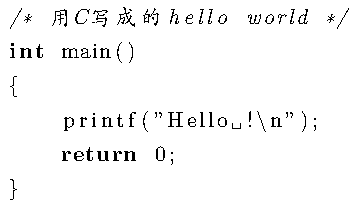
\includegraphics{texs/chelloworld1}
}
\begin{verbatim}
\begin{C}
    /* 用C写成的hello world */
    int main()
    {
        printf("Hello !\n");
        return 0;
    }
\end{C}\end{verbatim}
\end{codelist}

显然,有大量配置选项让你可以根据需要来调整该环境。想要了解它们,阅读包的文档无疑是最简单有效的。例如,我们可以修改相关编程语言中保留字和注释的版式。如此一来,我们就可以通过如下代码来实现不同的字体效果:

\begin{dmd}
\begin{verbatim}
\lstnewenvironment{Cbis}{% 
    \lstset{language=C,
        basicstyle=\rmfamily\slshape,
        commentstyle=\rmfamily\upshape,}}{}\end{verbatim}
\end{dmd}

\begin{codelist}[10.8]{
    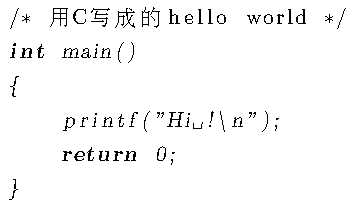
\includegraphics{texs/chelloworld2}
}
\begin{verbatim}
\begin{C}
    /* 用C写成的hello world */
    int main()
    {
        printf("Hello !\n");
        return 0;
    }
\end{C}\end{verbatim}
\end{codelist}

此外,因为还要考虑用于\emph{逃回\LaTeX }的特殊字符,你需要知道,正如\textsf{fancyvrb},包\textsf{listings}也允许你指定一个用于逃跑的字符:

\begin{dmd}
\begin{verbatim}
\lstnewenvironment{Cter}{% 
    \lstset{language=C, escapechar=@}}{}\end{verbatim}
\end{dmd}

以上代码在代码清单中插入\LaTeX 指令的效果如下:

\begin{codelist}[10.9]{
    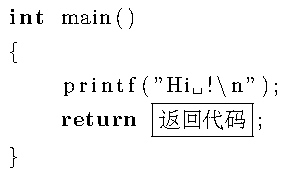
\includegraphics{texs/chelloworld3}
}
\begin{verbatim}
\begin{Cter}
    int main()
    {
        printf("Hi !\n");
        return @\fbox{返回代码}@;
    } 
\end{Cter}\end{verbatim}
\end{codelist}

\section{关于那个叫做``法文引号''的玩意儿}

法文排版的乐趣之一不容置疑地归属于卓越的``法国特色''引号的使用方式\jz{
    此外,我们注意到,现在很流行伸出食指和中指勾动来表示引号,但我们仍在使用代表法文引号``«''和``»''的guillet一词来表示引号。这种兔耳朵一样的手势无疑是从美国人那里传来的。因此,我公开呼吁,我们要使用拇指和食指来表示引号。然而,为了形象地模仿出法文引号这种双层尖角的特征,也许需要再长出两只胳膊,或习惯于扭动一只手的四根手指才行。
}……然而,我们在文档中输入法文引号时,包\textsf{babel}没法正确处理断字:

\begin{dmd}
\begin{verbatim}
\begin{minipage}{3.7cm}
    字盒中的这句话仅仅是为了去证明此处出现的法文引号处理得不够 « 优雅 »。
\end{minipage}\end{verbatim}
\end{dmd}

这个字盒的显示效果为:
\begin{minipage}{3.7cm}
    字盒中的这句话仅仅是为了去证明此处出现的法文引号处理得不够 « 优雅 »。
\end{minipage}

至少这种处理方式让人很不舒服……当然,可以借助包\textsf{babel}中的指令\verb|\og|和\verb|\fg|来插入法文引号,但依鄙人的品味,这种输入方式显得束手束脚,尤其是考虑到法文引号可以在法文键盘上直接输入\jz{
    分别使用\ovalbox{Alt Gr}+\ovalbox{Z}和\ovalbox{Alt Gr}+\ovalbox{X}快捷键。
}。一种曾经由包\textsf{french}适配的解决方案通过将字符``«''和``»''设为活跃\celan{\S 10.5.1}来缓解了断字的问题。因此,我们可以这样编写:

\begin{dmd}
\begin{verbatim}
\catcode`\«=13
\catcode`\»=13\end{verbatim}
\end{dmd}

然后定义以下两个指令:

\begin{dmd}
\begin{verbatim}
\newcommand{\fermerguillemets}{% 
\unskip\kern.15em\symbol{20}} 
\newcommand{\ouvrerguillemets}{%
\symbol{19}\ignorespaces\kern.15em}\end{verbatim}
\end{dmd}

注意到,此处使用了可以根据指定长度插入一段不可打断的空白的指令\TeX 指令\verb|\kern|,使用了指令\verb|\unskip|\celan{\S 9.2.1},还使用了指令\verb|\symbol|来插入当前字体中的第19和第20个字符:

\begin{codelist}[10.10]{
\newcounter{car}
\setcounter{car}{1}
\fontencoding{T1} \selectfont
\whiledo{\value{car}<64}{%
  \symbol{\value{car}}$_{\thecar}$
  \stepcounter{car}}
}
\begin{verbatim}
\setcounter{car}{1}
\whiledo{\value{car}<64}{%
  \symbol{\value{car}}$_{\thecar}$
  \stepcounter{car}}\end{verbatim}
\end{codelist}

最终,我们为这两个符号分配了前面的指令:

\begin{dmd}
\begin{verbatim}
\let»=\fermerguillemets
\let«=\ouvrerguillemets\end{verbatim}
\end{dmd}

\begin{qquestion}
这种操作方式有三个我仍然没法解决的小问题。首先,目前没有广泛流传的既能操作编码UTF-8,又能允许\TeX 将符号<<(编码为2字节)设置为活跃的引擎,我必须得谦卑地承认,我还没有测试它们。因此,这里提到的操作仅限于将每个字符编码为1字节的编码方式。其次,我们不能在标题中使用这些引号,因为可能有被识别为``书签''(signet;英:\emph{bookmark})的可能。最后,这些引号在第11章%TODO
末尾的环境\dm{ltxexemple}中无法使用。悲剧了!
\end{qquestion}

\section{用于微型摘要的字盒}

包\textsf{minitoc}可以生成``微型目录''(正如其名),以便我们在文档的指定位置插入。一般来说,我们会将微型摘要插在章首。在文前部分使用命令\verb|\dominitoc|之后,我们可以调用指令\verb|\minitoc|来在想要的位置插入这个微型目录。包的文档详细解释了相关信息,还介绍了我们可以使用的不同风格。对于本书,我为章首构思了一种十分漂亮的目录,但该包不支持其中涉及的风格。实际上,我曾希望以如下的方式将各节标题展示在一个方框中:

\begin{center}
    \titlebox{摘要}{%
        \begin{minipage}{0.5\linewidth}
            \begin{flushleft}
            \bfseries
            $\times $.1 标题一\\
            $\times $.2 标题二\\
            $\times $.3 等等
            \end{flushleft}
        \end{minipage}}
\end{center}

详细来说,这是一个带有标题的字盒,此处的标题是``摘要''。据我所知,\LaTeX 不提供这种字盒。我在论坛上提出这个问题后,一位好心人——邦雅曼·巴亚尔——为我提供了一段符合需求的代码。在本节,我会为你们提供一段用于生成带标题的字盒的\LaTeX 代码\jz{
    毫无疑问,这段代码值得商榷,且功能有限,就像哪些诞生于小作坊的``软件''一样……
}

\subsection{指令界面}

有多种方式可以创建此类指令。受\LaTeX 中字盒界面的灵感启发,我们可以使用这种语法来创建宏:

\begin{codelist}[10.11]{
    \titlebox{\footnotesize 标题}{%
  字盒中的内容}
}
\begin{verbatim}
\titlebox{\footnotesize 标题}{%
  字盒中的内容}\end{verbatim}
\end{codelist}

以及:

\begin{codelist}[10.12]{
    \setlength{\fboxsep}{5pt}
\setlength{\fboxrule}{2pt}
\titlebox{另一个标题}{%
\begin{minipage}{3cm}\begin{center} 
    一些东西\\ 一些玩意
\end{center}\end{minipage}}
}
\begin{verbatim}
\setlength{\fboxsep}{5pt}
\setlength{\fboxrule}{2pt}
\titlebox{另一个标题}{%
\begin{minipage}{3cm}\begin{center} 
    一些东西\\ 一些玩意
\end{center}\end{minipage}}\end{verbatim}
\end{codelist}

\subsection{还是得来点\TeX}

\TeX 原语\verb|\leaders|可以使用你想到的任何内容来填充一个弹性空间,语法如下:

\begin{dmd}
\verb|\leaders|\codereplace{随你喜欢}\codereplace{空间}
\end{dmd}

这样可以使用\codereplace{随你喜欢}来填满\codereplace{空间}。例如:

\begin{codelist}[10.13]{
\framebox[3cm]{%
  \leaders\hbox{o}\hfill}
}
\begin{verbatim}
\framebox[3cm]{%
    \leaders\hbox{o}\hfill}\end{verbatim}
\end{codelist}

\TeX 原语\verb|\hbox|(由\verb|\mbox|和\verb|\makebox|使用)可以创建水平字盒:

\begin{codelist}[10.14]{
\framebox[3cm]{%
    \leaders\hbox to 3pt{o}\hfill}
}
\begin{verbatim}
\framebox[3cm]{%
    \leaders\hbox to 3pt{o}\hfill}\end{verbatim}
\end{codelist}

\verb|\leaders|同样可以与\TeX 原语\verb|\hrule|结合,用来画线:

\begin{codelist}[10.15]{
\framebox[3cm]{%
    \leaders\hrule height 4pt\hfill}
}
\begin{verbatim}
\framebox[3cm]{%
    \leaders\hrule height 4pt\hfill}\end{verbatim}
\end{codelist}

这里,弹性长度\verb|\hfill|延展为\verb|\framebox|的3 cm,并由线宽为4 pt的线段填充。

\begin{codelist}[10.16]{
    \framebox[3cm]{%
    \leaders\hbox to5pt{%
      \leaders\hrule width1pt\hfill%
      \kern2pt}\hfill}
}
\begin{verbatim}
\framebox[3cm]{%
    \leaders\hbox to5pt{%
        \leaders\hrule width1pt\hfill%
        \kern2pt}\hfill}\end{verbatim}
\end{codelist}

在上述示例中,3 cm的空间被宽度为5 pt的字盒填充,每个字盒中包含如前展示的\verb|\leaders|,以及宽度为2 pt的空白。借助\TeX ,我们可以使用以下方式规范弹性长度的``僵硬''程度\celan{\S 4.2.4}:

\begin{codelist}[10.17]{
    \framebox[4cm]{%
    \hskip0pt plus 2fill X%
    \hskip0pt plus 3fill}
}
\begin{verbatim}
\framebox[4cm]{%
    \hskip0pt plus 2fill X%
    \hskip0pt plus 3fill}\end{verbatim}
\end{codelist}

其中,以下尺寸可以定义相对``僵硬''程度为$n$的弹性长度:

\begin{dmd}
\verb|\hskip 0pt plus |\codereplace{n}fill
\end{dmd}

\newcommand{\mafraction}[2]{%
\raisebox{0.5ex}{#1}%
\slash\raisebox{-0.5ex}{#2}}

因此,在上面的示例中,字母``X''出现在字盒中\mafraction{2}{5}的位置……使用此类的弹性空白和\verb|\leaders|,我们可以定义出如下的内容并在以下示例中使用:

\begin{dmd}
\begin{verbatim}
\newcommand{\traitressort}[2][1]{%
    \leaders\hrule height#2\hskip0pt plus #1fill\relax}\end{verbatim}
\end{dmd}

\begin{codelist}[10.18]{
    \framebox[4cm]{%
    \traitressort[2]{2ex}X%
    \traitressort{2pt}}
}
\begin{verbatim}
\framebox[4cm]{%
    \traitressort[2]{2ex}X%
    \traitressort{2pt}}\end{verbatim}
\end{codelist}

在该5 cm宽的字盒中,我们有:

\begin{itemize}
    \item ``僵硬''程度为2的弹性空白,由线宽为4 pt的线段填充;
    \item 字母X;
    \item ``僵硬''程度为1的弹性空白,由线宽为2 pt的线段填充;
\end{itemize}

接下来,我们将很快得到该指令为我们服务的消息……

\subsection{字盒的概念}

为了构建我们需要的那种字盒,我们将要按如下方式创建三个字盒:

\begin{center}
    \fbox{\parbox{3pt}{%
        \rule{0pt}{1.215cm}%
        \rule{3pt}{1.025cm}}}%
    \parbox[][1.5cm][c]{4cm}{%
        \begin{flushleft}
          \framebox[4cm]{%
            \traitressort{3pt}
            \raisebox{-.23ex}{标题}
            \traitressort[4]{3pt}}\\\nointerlineskip
          \framebox[4cm]{内容}\\\nointerlineskip
          \framebox[4cm]{\traitressort{3pt}}
        \end{flushleft}}%
    \fbox{\parbox{3pt}{%
        \rule{0pt}{1.215cm}%
        \rule{3pt}{1.025cm}}}
\end{center}

其中包含:

\begin{itemize}
    \item 两个\verb|\parbox|,用于包含左右两侧的竖线;
    \item 中央的一个\verb|\parbox|,包含响应标题变化的横线、内容,以及底部的水平线。
\end{itemize}

很快,我们就会看到如何构建这三个字盒,并且一个参考一个地放置它们。

\subsection{代码}

我们需要一个字盒来存储位于中央的\verb|\parbox|:

\begin{dmd}
\verb|\newsavebox{\boitetitre}|
\end{dmd}

还需要两个尺寸:

\begin{dmd}
\begin{verbatim}
\newlength{\largeurboitetitre}
\newlength{\hauteurboitetitre}\end{verbatim}
\end{dmd}

尺寸的名称十分具体\yz{
    分别指标题字盒(boîte titre)的宽度(largeur)和高度(hauteur)。
},因此,我不必去组织那些晦涩的句子来解释这个或那个变量的含义。我们要求指令\verb|\titlebox|做的第一个任务是存储并测量其内容的尺寸:

\begin{dmd}
\begin{verbatim}
\newcommand{\titlebox}[2]{% 
    \begin{lrbox}{\boitetitre}% 存储内容
        \kern\fboxsep#2\kern\fboxsep
    \end{lrbox}
    % 测量该中央段落字盒的宽度 
    \settowidth{\largeurboitetitre}{\usebox{\boitetitre}}% 
    % 测量该中央段落字盒的高度
    \settoheight{\hauteurboitetitre}{\usebox{\boitetitre}}% 
    \settodepth{\tempdim}{\usebox{\boitetitre}}% 
    \addtolength{\hauteurboitetitre}{%
        \tempdim+2\fboxrule+2\fboxsep}%
    ... }\end{verbatim}
\end{dmd}

\verb|\kern|是\TeX 指令,用于插入可插入的空白,此处为宽度\verb|\fboxsep|。注意,为了测量总高度,我们借助了一个求高度(\emph{英:height})和深度(\emph{英:depth})之和的临时长度。接下来,我们在该总高度的基础上添加了两倍的线宽和两倍的空间\verb|\fboxsep|。回忆一下,尺寸\verb|\fboxrule|和\verb|\fboxsep|分别定义了线宽和简单字盒\celan{\S 4.4.1}内容和边框间的空间。因此,我们有:

\begin{itemize}
    \item \verb|\largeurboitetitre|代表了中央\verb|\parbox|的宽度和二倍\verb|\fboxsep|的和;
    \item \verb|\hauteurboitetitre|代表了计入两条水平线线宽后的总高度\verb|2(\fboxsep+\fboxrule)|。
\end{itemize}

因此,我们可以搭建第一版指令:

\begin{dmd}
\begin{verbatim}
\newcommand{\titleboxI}[2]{% 
    ...
    \parbox{\fboxrule}{% 左侧线段
        \rule{\fboxrule}{\hauteurboitetitre}}%
    \parbox{\largeurboitetitre}{% 中央字盒
        \begin{flushleft}
            \usebox{\boitetitre} 
        \end{flushleft}}%
    \parbox{\fboxrule}{% 右侧线段
        \rule{\fboxrule}{\hauteurboitetitre}}}}\end{verbatim}
\end{dmd}

\newcommand{\titleboxI}[2]{%
  \begin{lrbox}{\boitetitre}% stockage du contenu
    \kern\fboxsep#2\kern\fboxsep
  \end{lrbox}
  % mesure de la largeur de la parbox centrale
  \settowidth{\largeurboitetitre}{\usebox{\boitetitre}}%
  % mesure de la hauteur de la parbox centrale
  \settoheight{\hauteurboitetitre}{\usebox{\boitetitre}}%
  \settodepth{\tempdim}{\usebox{\boitetitre}}%
  \addtolength{\hauteurboitetitre}{\tempdim+2\fboxrule+2\fboxsep}%
  \parbox{\fboxrule}{%
    \rule{\fboxrule}{\hauteurboitetitre}}%
  \parbox{\largeurboitetitre}{%
    \begin{flushleft}
      \usebox{\boitetitre}
    \end{flushleft}}%
  \parbox{\fboxrule}{%
    \rule{\fboxrule}{\hauteurboitetitre}}}

目前,其效果为:

\begin{codelist}[10.19]{
    \titleboxI{titre}{一些东西二些东西}

\titleboxI{encore}{%
  \parbox{4cm}{东西\\玩意\\零七八碎}}
}
\begin{verbatim}
\titleboxI{titre}{一些东西二些东西}

\titleboxI{encore}{%
  \parbox{4cm}{东西\\玩意\\零七八碎}}\end{verbatim}
\end{codelist}

接下来要做的是修改中央\verb|\parbox|的内容,以加入两条水平线——下方的线段和上方被标题打断的线段。这里的思路是堆叠三个字盒:

\begin{enumerate}
    \item 包含标题和``弹性线段''的字盒;
    \item 存储内容(\verb|\boitetitre|)的字盒;
    \item 宽度为\verb|\largeurboitetitre|的线段。
\end{enumerate}

我们的第一次尝试如下:

\begin{dmd}
\begin{verbatim}
\newcommand{\titleboxII}[2]{% 
    ...
    \parbox{\largeurboitetitre}{% 中央字盒
        \begin{flushleft}
            \makebox[\largeurboitetitre]{% 
                \traitressort{\fboxrule}#1% 
                \traitressort[5]{\fboxrule}}\\
            \usebox{\boitetitre}\\
            \rule{\largeurboitetitre}{\fboxrule}
        \end{flushleft}}
    ...}\end{verbatim}
\end{dmd}

\newcommand{\titleboxII}[2]{%
  \begin{lrbox}{\boitetitre}% stockage du contenu
    \kern\fboxsep#2\kern\fboxsep
  \end{lrbox}
  % mesure de la largeur de la parbox centrale
  \settowidth{\largeurboitetitre}{\usebox{\boitetitre}}%
  % mesure de la hauteur de la parbox centrale
  \settoheight{\hauteurboitetitre}{\usebox{\boitetitre}}%
  \settodepth{\tempdim}{\usebox{\boitetitre}}%
  \addtolength{\hauteurboitetitre}{\tempdim+2\fboxrule+2\fboxsep}%
  \parbox{\fboxrule}{%
    \rule{\fboxrule}{\hauteurboitetitre}}%
  \parbox{\largeurboitetitre}{%
    \begin{flushleft}
      \makebox[\largeurboitetitre]{%
        \traitressort{\fboxrule}#1\traitressort[5]{\fboxrule}}\\
      \usebox{\boitetitre}\\
      \rule{\largeurboitetitre}{\fboxrule}
    \end{flushleft}}%
  \parbox{\fboxrule}{%
    \rule{\fboxrule}{\hauteurboitetitre}}}

效果如下:

\begin{codelist}[10.20]{
    \titleboxII{标题}{一些东西二些东西}

    \titleboxII{再来一个}{%
        \parbox{4cm}{零七\\八碎}}
}
\begin{verbatim}
\titleboxII{标题}{一些东西二些东西}

\titleboxII{再来一个}{%
    \parbox{4cm}{零七\\八碎}}\end{verbatim}
\end{codelist}

可以说,这``不完全''是我们想要的。接下来需要考虑的是尽量让指令\verb|\\|实现竖直方向上与尺寸\verb|\fboxsep|相同的换行。我们可以顺便让标题竖直向下移动,来实现这一点:

\begin{dmd}
\begin{verbatim}
\newcommand{\titleboxIII}[2]{%
    ...
    \parbox{\largeurboitetitre}{% 中央字盒
        \begin{flushleft}
        \makebox[\largeurboitetitre]{%
            \traitressort{\fboxrule}%
            \raisebox{-.5ex}[0pt][0pt]{#1}%
            \traitressort[5]{\fboxrule}}\\[\fboxsep]
        \usebox{\boitetitre}\\[\fboxsep]
        \rule{\largeurboitetitre}{\fboxrule}
        \end{flushleft}}  
    ...}\end{verbatim}
\end{dmd}

\newcommand{\titleboxIII}[2]{%
  \begin{lrbox}{\boitetitre}% stockage du contenu
    \kern\fboxsep#2\kern\fboxsep
  \end{lrbox}
  % mesure de la largeur de la parbox centrale
  \settowidth{\largeurboitetitre}{\usebox{\boitetitre}}%
  % mesure de la hauteur de la parbox centrale
  \settoheight{\hauteurboitetitre}{\usebox{\boitetitre}}%
  \settodepth{\tempdim}{\usebox{\boitetitre}}%
  \addtolength{\hauteurboitetitre}{\tempdim+2\fboxrule+2\fboxsep}%
  \parbox{\fboxrule}{%
    \rule{\fboxrule}{\hauteurboitetitre}}%
  \parbox{\largeurboitetitre}{%
    \begin{flushleft}
      \makebox[\largeurboitetitre]{%
        \traitressort{\fboxrule}%
        \raisebox{-.5ex}[0pt][0pt]{#1}%
        \traitressort[5]{\fboxrule}}\\[\fboxsep]
      \usebox{\boitetitre}\\[\fboxsep]
      \rule{\largeurboitetitre}{\fboxrule}
    \end{flushleft}}%
  \parbox{\fboxrule}{%
    \rule{\fboxrule}{\hauteurboitetitre}}}

效果为:

\begin{codelist}[10.21]{
    \titleboxIII{标题}{一些东西二些东西}

\titleboxIII{再来一个}{%
    \parbox{4cm}{零七\\八碎}}
}
\begin{verbatim}
\titleboxIII{标题}{一些东西二些东西}

\titleboxIII{再来一个}{%
    \parbox{4cm}{零七\\八碎}}\end{verbatim}
\end{codelist}

可以说规整得没什么效果……需要知道,当\TeX 在纵向模式下堆叠字盒是,它本身就会在字盒间插入空间,来保证行间距为长度\verb|\baselineskip|。在\TeX Book的79页有关处理\emph{glue}的章节中,我们可以找到:

\begin{origincitation}[高德纳,\TeX Book{[9]}]
    例外情况:线段字盒的前后不会插入用于跨行分隔的垫胶。你也可以通过在两个字盒间插入\verb|\nointerlineskip|来禁用垫胶。
\end{origincitation}

因此,命令\verb|\nointerlineskip|可以解决这个问题:

\begin{dmd}
\begin{verbatim}
\newcommand{\titleboxIV}[2]{%
    ...
    \parbox{\largeurboitetitre}{% 中央字盒
        \begin{flushleft}
        \makebox[\largeurboitetitre]{%
            \traitressort{\fboxrule}%
            \raisebox{-.5ex}[0pt][0pt]{#1}%
            \traitressort[5]{\fboxrule}}\\[\fboxsep]
        \nointerlineskip
        \usebox{\boitetitre}\\[\fboxsep]\nointerlineskip
        \rule{\largeurboitetitre}{\fboxrule}
        \end{flushleft}}  
    ...}\end{verbatim}
\end{dmd}

\newcommand{\titleboxIV}[2]{%
  \begin{lrbox}{\boitetitre}% stockage du contenu
    \kern\fboxsep#2\kern\fboxsep
  \end{lrbox}
  % mesure de la largeur de la parbox centrale
  \settowidth{\largeurboitetitre}{\usebox{\boitetitre}}%
  % mesure de la hauteur de la parbox centrale
  \settoheight{\hauteurboitetitre}{\usebox{\boitetitre}}%
  \settodepth{\tempdim}{\usebox{\boitetitre}}%
  \addtolength{\hauteurboitetitre}{\tempdim+2\fboxrule+2\fboxsep}%
  \parbox{\fboxrule}{%
    \rule{\fboxrule}{\hauteurboitetitre}}%
  \parbox{\largeurboitetitre}{%
    \begin{flushleft}
      \makebox[\largeurboitetitre]{%
        \traitressort{\fboxrule}%
        \raisebox{-.5ex}[0pt][0pt]{#1}%
        \traitressort[5]{\fboxrule}}\\[\fboxsep]\nointerlineskip
      \usebox{\boitetitre}\\[\fboxsep]\nointerlineskip
      \rule{\largeurboitetitre}{\fboxrule}
    \end{flushleft}}%
  \parbox{\fboxrule}{%
    \rule{\fboxrule}{\hauteurboitetitre}}}
\enlargethispage{2cm}

效果为:

\begin{codelist}[10.22]{
\titleboxIV{标题}{一些东西二些东西}

\titleboxIV{再来一个}{%
    \parbox{4cm}{零七\\八碎}}
}
\begin{verbatim}
\titleboxIV{标题}{一些东西二些东西}

\titleboxIV{再来一个}{%
    \parbox{4cm}{零七\\八碎}}\end{verbatim}
\end{codelist}

这样就满足了我们的需求。

\begin{ii}
这个指令还有很多可以完善的地方,我把它们留作练习。例如,我们可以定义一个可选的参数,来规定标题下沉的程度(目前我们强制其为\dm{-0.5ex})。同样,也可以规定标题周围线段的比例。最后,也当然可以考虑规定标题周围的空间(此处没有留空间)。
\end{ii}

\subsection{借助包\textsf{minitoc}的应用}

使用前文中定义的指令\verb|\titlebox|,包\textsf{minitoc}中发生的事情只是简单地戴上波洛先生的帽子。通过仔细检查风格文件,我们找到了一个叫做\verb|\minitoc@|的指令的定义。我只是简单地将这个宏的代码照抄了下来,并且在卓越的指令\verb|\titlebox|中加入了一次调用。

